\documentclass[a4paper]{article}

% \usepackage[spanish]{babel}
% \usepackage[utf8x]{inputenc}
\usepackage{pgf}
\usepackage{tikz}
\usetikzlibrary{arrows,automata}
\usepackage{amsmath}
\usepackage{amsfonts}
\usepackage{amssymb}
\usepackage{amsmath}
\usepackage{amscd}
% \usepackage{esint}
% \usepackage{bbold}
\usepackage{graphicx}
\usepackage{slashed}

% \usepackage[colorinlistoftodos]{todonotes}
\addtolength{\oddsidemargin}{-.875in}
\addtolength{\evensidemargin}{-.875in}
\addtolength{\textwidth}{1.70in}
\addtolength{\topmargin}{-.875in}
\addtolength{\textheight}{1.50in}

\def \Int#1{\int d#1 \hskip0.1cm}

\def \FNode{ \texttt{FNode} }
\def \FNodes{ \texttt{FNodes} }
\def \FLink{ \texttt{FLink} }
\def \FLinks{ \texttt{FLinks} }


\title{Color Handling @\texttt{NLOX}}
\author{Diógenes Figueroa}
\begin{document}
% \date{Febrero 17 de 2017}
\maketitle
\section{Topological Color}
In this section we will discuss the method by which \texttt{NLOX} handles color matrices to reduce the number 
of evaluations of color traces. The general scheme is to recursively apply the following set of identities:

\begin{itemize}
 \item $f^{a_1a_2a_3} = -2i(Tr(T^{a_1} T^{a_2} T^{a_3})-Tr(T^{a_1} T^{a_3} T^{a_2}))$
 \item $(T^a)_{i_1i_2}(T^a)_{i_3i_4} = \frac{1}{2}\left(\delta_{i_1i_4}\delta_{i_2i_3} - \frac{1}{Nc}\delta_{i_1i_2}\delta_{i_3i_4}\right)$
 \item $Tr(T^a) = 0$
 \item $Tr(T^{a_1}T^{a_2})=\frac{1}{2}\delta^{a_1 a_2}$
\end{itemize}

This will fully simplify any sequence of $f$ tensors and $T$ matrices down to (possibly) traces of $T$ matrices.
For fully contracted sequences the result will be a number. 

\subsection{On the redundancy of the $f-T$ representation}
Let's consider the example of sequences of $8$ fully contracted $f$ tensors, there are in principle $12!$ such sequences one might encounter, however if we make full use of the anti-symmetry of the $f$ tensors it turns out there are only $12$ independent structures. To understand how can we identify such independant structures we have to change perspective, we identify every $f$ tnesor with an \texttt{FNode} which can connect to $3$ other \texttt{FNodes}.
Two \texttt{FNodes} are connected if they share an index. In our example of $8$ fully contracted $f$ tensors 
every node is connected to $3$ other \texttt{FNodes}.
To further simplify the \texttt{FNode} expressions we make use of the identities:
\begin{itemize}
 \item $f^{a_1 a_2 a_3} f^{a_1a_2a_4} = C_A \delta^{a_3a_4}$
 \item $f^{a_1 a_2 a_3} f^{a_1a_2a_3} = N_A C_A $
\end{itemize}
what this does is it makes sure that there are either $0$ or $1$ links between any two \texttt{FNodes}.
We are ready to introduce the concept of a \texttt{FFLink}, if two \texttt{FNodes} share an index on the 
same position we say they form a \texttt{FFLink}, is they share an index but they are not in the same position
we use the anti-symmetry of the $f$ to move one of them so it coincides with the other $f$, and pay the appropiate
sign if necessary. Let's work out a simple example, consider:

\begin{equation}
\begin{aligned}
 f^{a_1a_2a_3}f^{a_4a_5a_6}f^{a_7a_8a_9}f^{a_1a_4a_7}f^{a_2a_5a_8}f^{a_3a_6a_9}
 \rightarrow
 &\texttt{FNode}(a_1,a_2,a_3;1)\texttt{FNode}(a_4,a_5,a_6;5)\texttt{FNode}(a_7,a_8,a_9;6)\\
 &\texttt{FNode}(a_1,a_4,a_7;2)\texttt{FNode}(a_2,a_5,a_8;3)\texttt{FNode}(a_3,a_6,a_9;4)\\
 \rightarrow
 &\texttt{FFLink}(1,2)\texttt{FFLink}(1,3)\texttt{FFLink}(1,4)\\
 &\texttt{FFLink}(5,2)\texttt{FFLink}(5,3)\texttt{FFLink}(5,4)\\
 &\texttt{FFLink}(6,2)\texttt{FFLink}(6,3)\texttt{FFLink}(6,4)\\
 \end{aligned}
\end{equation}
the \texttt{FNode} numbering is arbitrary and hence we have the freedom to choose, however, 
since we want to classify the different sequences of $f$, it is desirable to have a cannonical 
naming scheme in which the equivalence between sequences is manifest. For example one might pick a 
\texttt{FNode} and call it $\#1$, then it is natural to define the \texttt{FNodes} $\#2$, $\#3$ and $\#4$ as simpliy those connected to $\#1$, we know they are all different since any \texttt{FNode} has only 
one connection with any other. This is as far as general structures go, but we can continue labeling our 
graph using lexicographical ordering and this procedure fully idntifies equivalent structures under full
anti-symmetry of the $f$ tensor. 

\subsection{Colored Graphs}
A better way for understanding what the \texttt{FNodes} and \texttt{FFLinks} are refering to is to 
associate diagrams with each one, for a $\texttt{FNode}(a_1,a_2,a_3,;1)$, we draw:

\begin{center}
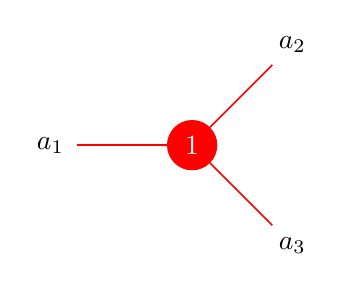
\begin{tikzpicture}[>=stealth',shorten >=1pt,auto,node distance=1.8cm,
                    semithick]
  \tikzstyle{every state}=[fill=red,draw=red,text=white,minimum size=5mm]

  \node[state] (1)                   {$1$};
  \node(a1)    [left of=1]           {$a_1$};
  \node(a2)    [above right of=1]    {$a_2$};
  \node(a3)    [below right of=1]    {$a_3$};
  \draw[red] 
        (1) edge              node {} (a1)
            edge              node {} (a2)
            edge              node {} (a3);
\end{tikzpicture}
\end{center}
the identity $f^{a_1 a_2 a_3} f^{a_1a_2a_4} = C_A \delta^{a_3a_4}$ corresponds to:
\begin{center}
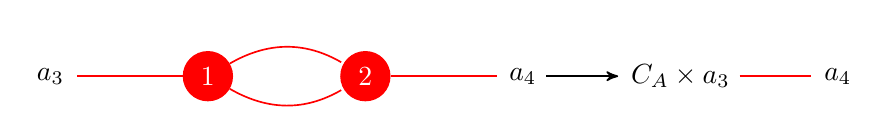
\begin{tikzpicture}[>=stealth',shorten >=1pt,auto,node distance=2cm,
                    semithick]
  \tikzstyle{every state}=[fill=red,draw=red,text=white,minimum size=5mm]

  \node[state] (1)                   {$1$};
  \node(a1)    [left of=1]           {$a_3$};
  \node[state] (2) [right of=1]      {$2$};
  \node(a2)    [right of=2]           {$a_4$};
  \draw[red] 
        (1) edge   [bend right]         node {} (2)
        (1) edge   [bend left]          node {} (2)
        (1) edge node {} (a1)
        (2) edge node {} (a2);
  \node (a3) [right of=a2] {$C_A\times a_3$};
  \node (a4) [right of=a3] {$a_4$};
  \draw[black,->] 
  (a2) edge node{} (a3);
  \draw[red]
  (a3) edge node{} (a4);
\end{tikzpicture}
\end{center}

The \texttt{FFLinks} correspond to the edges of the graphs, in terms of graphs the equivalence becomes, that two expressions are equivalent if they have the same graph. Our example has the corresponding graph:

\begin{center}
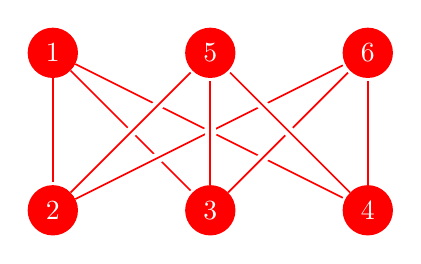
\begin{tikzpicture}[>=stealth',shorten >=1pt,auto,node distance=2cm,
                    semithick]
  \tikzstyle{every state}=[fill=red,draw=red,text=white,minimum size=5mm]

  \node[state] (1)                   {$1$};
  \node[state] (2) [below of=1]      {$2$};
  \node[state] (3) [right of=2]      {$3$};
  \node[state] (4) [right of=3]      {$4$};
  \node[state] (5) [right of=1]      {$5$};
  \node[state] (6) [right of=5]      {$6$};
  
  \draw[red] 
        (1) edge   [draw=white,double=red,double distance = \pgflinewidth,ultra thick]    node {} (2)
        (1) edge   [draw=white,double=red,double distance = \pgflinewidth,ultra thick]    node {} (3)
        (1) edge   [draw=white,double=red,double distance = \pgflinewidth,ultra thick]    node {} (4)
        (2) edge   [draw=white,double=red,double distance = \pgflinewidth,ultra thick]    node {} (5)
        (2) edge   [draw=white,double=red,double distance = \pgflinewidth,ultra thick]    node {} (6)
        (3) edge   [draw=white,double=red,double distance = \pgflinewidth,ultra thick]    node {} (5)
        (3) edge   [draw=white,double=red,double distance = \pgflinewidth,ultra thick]    node {} (6)
        (4) edge   [draw=white,double=red,double distance = \pgflinewidth,ultra thick]    node {} (5)
        (4) edge   [draw=white,double=red,double distance = \pgflinewidth,ultra thick]    node {} (6);
\end{tikzpicture}
\end{center}

this is the well-known bipartite graph $K_{3,3}$, the actual value of this graph is $0$. From now on we shall drop 
the labeling over the \FNodes, since the value of the grapsh is independent on this labeling. The relative spatial
possition of the nodes is also irrelevant for the value of the graph, for example the two graphs:

\begin{center}
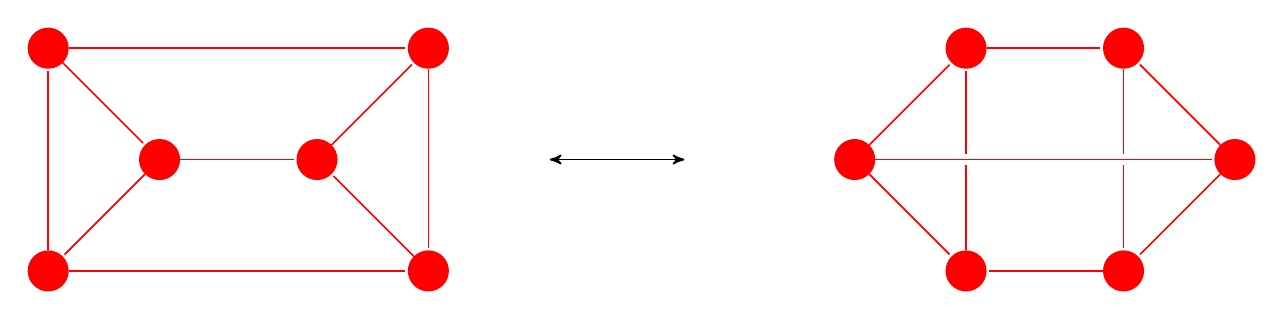
\begin{tikzpicture}[>=stealth',shorten >=1pt,auto,node distance=2cm,
                    semithick]
  \tikzstyle{every state}=[fill=red,draw=red,minimum size=5mm]

  \node[state] (1)                   {};
  \node[state] (2) [below left of=1]      {};
  \node[state] (3) [above left of=1]      {};
  \node[state] (4) [right of=1]      {};
  \node[state] (5) [above right of=4]      {};
  \node[state] (6) [below right of=4]      {};
  \node[] (G1) [below right of=5] {};
  
  \draw[red] 
        (1) edge   []         node {} (2)
        (2) edge   []         node {} (3)
        (3) edge   []         node {} (1)
        (1) edge   []         node {} (4)
        (2) edge   []         node {} (6)
        (3) edge   []         node {} (5)
        (4) edge   []         node {} (5)
        (5) edge   []         node {} (6)
        (6) edge   []         node {} (4);
  \node[] (G2) [right of=G1]{}; 
  \node[state] (7) [right of=G2]                {};
  \node[state] (8) [above right of=7]      {};
  \node[state] (9) [below right of=7]      {};
  \node[state] (10) [right of=8]      {};
  \node[state] (11) [right of=9]      {};
  \node[state] (12) [below right of=10]      {};
%   \node[state] (aux) [below right of=9]{};
  
  \draw[red] 
        (8) edge   []         node {} (10)
        (10) edge   []         node {} (11)
        (11) edge   []         node {} (9)
        (9) edge   []         node {} (8)
        (7) edge   []         node {} (8)
        (7) edge   []         node {} (9)
        (12) edge   []         node {} (10)
        (12) edge   []         node {} (11)
        (7) edge   [draw=white,double=red,double distance = \pgflinewidth,ultra thick] node {} (12);
  
  \draw[black,<->]
        (G1) edge node{}(G2);
\end{tikzpicture}
\end{center}

have the same value.

\subsection{Expression Classification using Graphs}
We now proceed to describe the classification procedure and how it is currently implemented in \texttt{NLOX}.
Graphs with only two nodes are evaluated down to a number trivially by the rules given in \eqref{}, so to start
we consider expressions with $4$ $f$ tensors, as we described before there is only one such strcture upon cannonical ordering, which is the tetrahedral graph:


\begin{center}
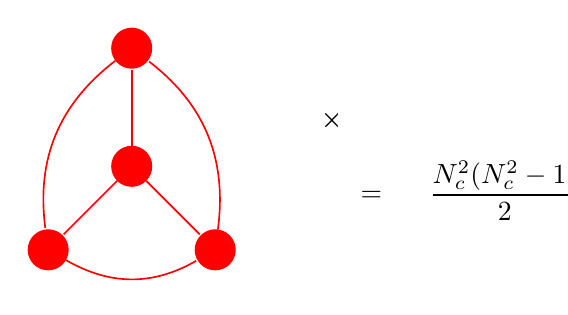
\begin{tikzpicture}[>=stealth',shorten >=0.5pt,auto,node distance=1.5cm,
                    semithick]
  \tikzstyle{every state}=[fill=red,draw=red,minimum size=5mm]
  \tikzstyle{equation} = [
    rectangle, rounded corners, inner sep=10pt, inner ysep=20pt]
  \node[state] (1)                   {};
  \node[state] (2) [above of=1]      {};
  \node[state] (3) [below left  of=1]      {};
  \node[state] (4) [below right of=1]      {};
  \node[] (Separator) [above right of=4]      {};
  \node[equation] (Value) [right of=Separator] {\begin{minipage}[ht!]{0.2\textwidth}
                                               ×\begin{equation*}
                                                   \hskip0.5cm =\hskip0.5cm  \frac{N_c^2(N_c^2-1)}{2}
                                                \end{equation*}
                                              \end{minipage}};
  \draw[red]
  (1) edge node{} (2)
  (1) edge node{} (3)
  (1) edge node{} (4)
  (2) edge [bend right]node{} (3)
  (3) edge [bend right]node{} (4)
  (4) edge [bend right]node{} (2);
  \end{tikzpicture}
\end{center}

for exprssions with $6$ \FNodes there are only $2$ possible graphs that are not trivially reduced to the tetrahedral graph, $K_{3,3}$ and the triangular prism graph shown above:

\begin{center}
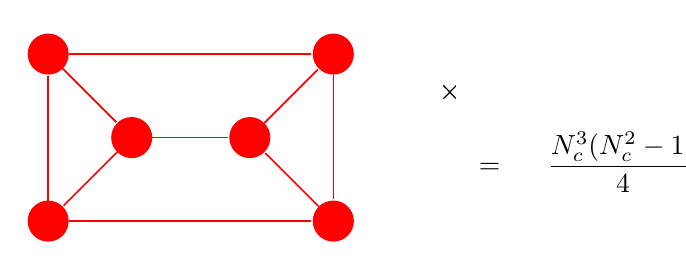
\begin{tikzpicture}[>=stealth',shorten >=0.5pt,auto,node distance=1.5cm,
                    semithick]
  \tikzstyle{every state}=[fill=red,draw=red,minimum size=5mm]
  \tikzstyle{equation} = [
    rectangle, rounded corners, inner sep=10pt, inner ysep=20pt]
  

  \node[state] (1)                   {};
  \node[state] (2) [below left of=1]      {};
  \node[state] (3) [above left of=1]      {};
  \node[state] (4) [right of=1]      {};
  \node[state] (5) [above right of=4]      {};
  \node[state] (6) [below right of=4]      {};
  \draw[red] 
        (1) edge   []         node {} (2)
        (2) edge   []         node {} (3)
        (3) edge   []         node {} (1)
        (1) edge   []         node {} (4)
        (2) edge   []         node {} (6)
        (3) edge   []         node {} (5)
        (4) edge   []         node {} (5)
        (5) edge   []         node {} (6)
        (6) edge   []         node {} (4);

  \node[] (Separator) [above right of=6]      {};
  \node[equation] (Value) [right of=Separator] {\begin{minipage}{0.2\textwidth}
                                               ×\begin{equation*}
                                                   \hskip0.5cm =\hskip0.5cm \frac{N_c^3(N_c^2-1)}{4}
                                                \end{equation*}
                                              \end{minipage}};
\end{tikzpicture}  
\end{center}

\begin{center}
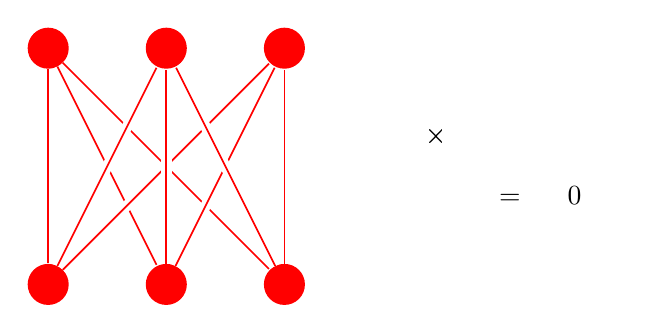
\begin{tikzpicture}[>=stealth',shorten >=0.5pt,auto,node distance=1.5cm,
                    semithick]
  \tikzstyle{every state}=[fill=red,draw=red,minimum size=5mm]
  \tikzstyle{equation} = [
    rectangle, rounded corners, inner sep=10pt, inner ysep=20pt]
  

  \node[state] (1){};
  
  \node[] (2B) [below of=1]      {};
  \node[state] (2) [below of=2B]      {};
  
  \node[state] (3) [right of=2]      {};
  \node[] (3B) [above of=3]      {};
  
  \node[state] (4) [right of=3]      {};
  \node[] (4B) [above of=4]      {};
  
  \node[state] (5) [right of=1]      {};
  \node[state] (6) [right of=5]      {};
  
  \draw[red] 
        (1) edge   [draw=white,double=red,double distance = \pgflinewidth,ultra thick]   node {} (2)
        (1) edge   [draw=white,double=red,double distance = \pgflinewidth,ultra thick]   node {} (3)
        (1) edge   [draw=white,double=red,double distance = \pgflinewidth,ultra thick]   node {} (4)
        (2) edge   [draw=white,double=red,double distance = \pgflinewidth,ultra thick]   node {} (5)
        (2) edge   [draw=white,double=red,double distance = \pgflinewidth,ultra thick]   node {} (6)
        (3) edge   [draw=white,double=red,double distance = \pgflinewidth,ultra thick]   node {} (5)
        (3) edge   [draw=white,double=red,double distance = \pgflinewidth,ultra thick]   node {} (6)
        (4) edge   [draw=white,double=red,double distance = \pgflinewidth,ultra thick]   node {} (5)
        (4) edge   [draw=white,double=red,double distance = \pgflinewidth,ultra thick]   node {} (6);
  \node[] (Separator) [right of=4B]      {};
  \node[equation] (Value) [right of=Separator] {\begin{minipage}{0.2\textwidth}
                                               ×\begin{equation*}
                                                   \hskip0.5cm =\hskip0.5cm 0
                                                \end{equation*}
                                              \end{minipage}};
\end{tikzpicture}  
\end{center}

while for $8$ \FNodes we have the structures:
\begin{center}
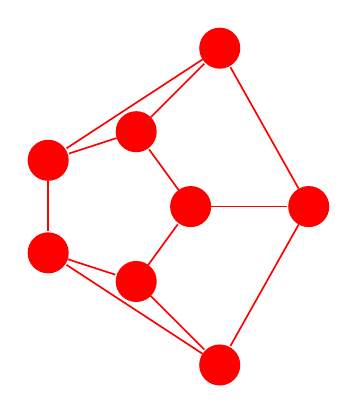
\begin{tikzpicture}[>=stealth',shorten >=0.5pt,auto,node distance=1.5cm,
                    semithick]
  \tikzstyle{every state}=[fill=red,draw=red,minimum size=5mm]
  \tikzstyle{equation} = [
    rectangle, rounded corners, inner sep=10pt, inner ysep=20pt]
  \node[] at (0,0) [] {};
  \node[state] (1) at (1,0) [] {};
  \node[state] (2) at (0.3090,0.9510) [] {};
  \node[state] (3) at (-0.809017, 0.587785) [] {};
  \node[state] (4) at (-0.809017, -0.587785) [] {};
  \node[state] (5) at (0.3090,-0.9510) [] {};
  \node[state] (6) [right of=1] {};
  \node[state] (7) [above right of=2] {};
  \node[state] (8) [below right of=5] {};
  \draw[red] 
        (1) edge  node {} (2)
        (2) edge  node {} (3)
        (3) edge  node {} (4)
        (4) edge  node {} (5)
        (5) edge  node {} (1)
        (1) edge  node {} (6)
        (2) edge  node {} (7)
        (5) edge  node {} (8)
        (6) edge  node {} (7)
        (6) edge  node {} (8)
        (7) edge  node {} (3)
        (8) edge  node {} (4);
     
  

  \end{tikzpicture}  
\end{center}












\end{document}
